%! Author = lili
%! Date = 4/22/26

\section{Auftrennung von doppelsträngiger DNA}\label{sec:auftrennung-von-doppelstrangiger-dna}
\frage{dnatrennung}

\begin{figure}[H]
    % TODO Schmelzkurve 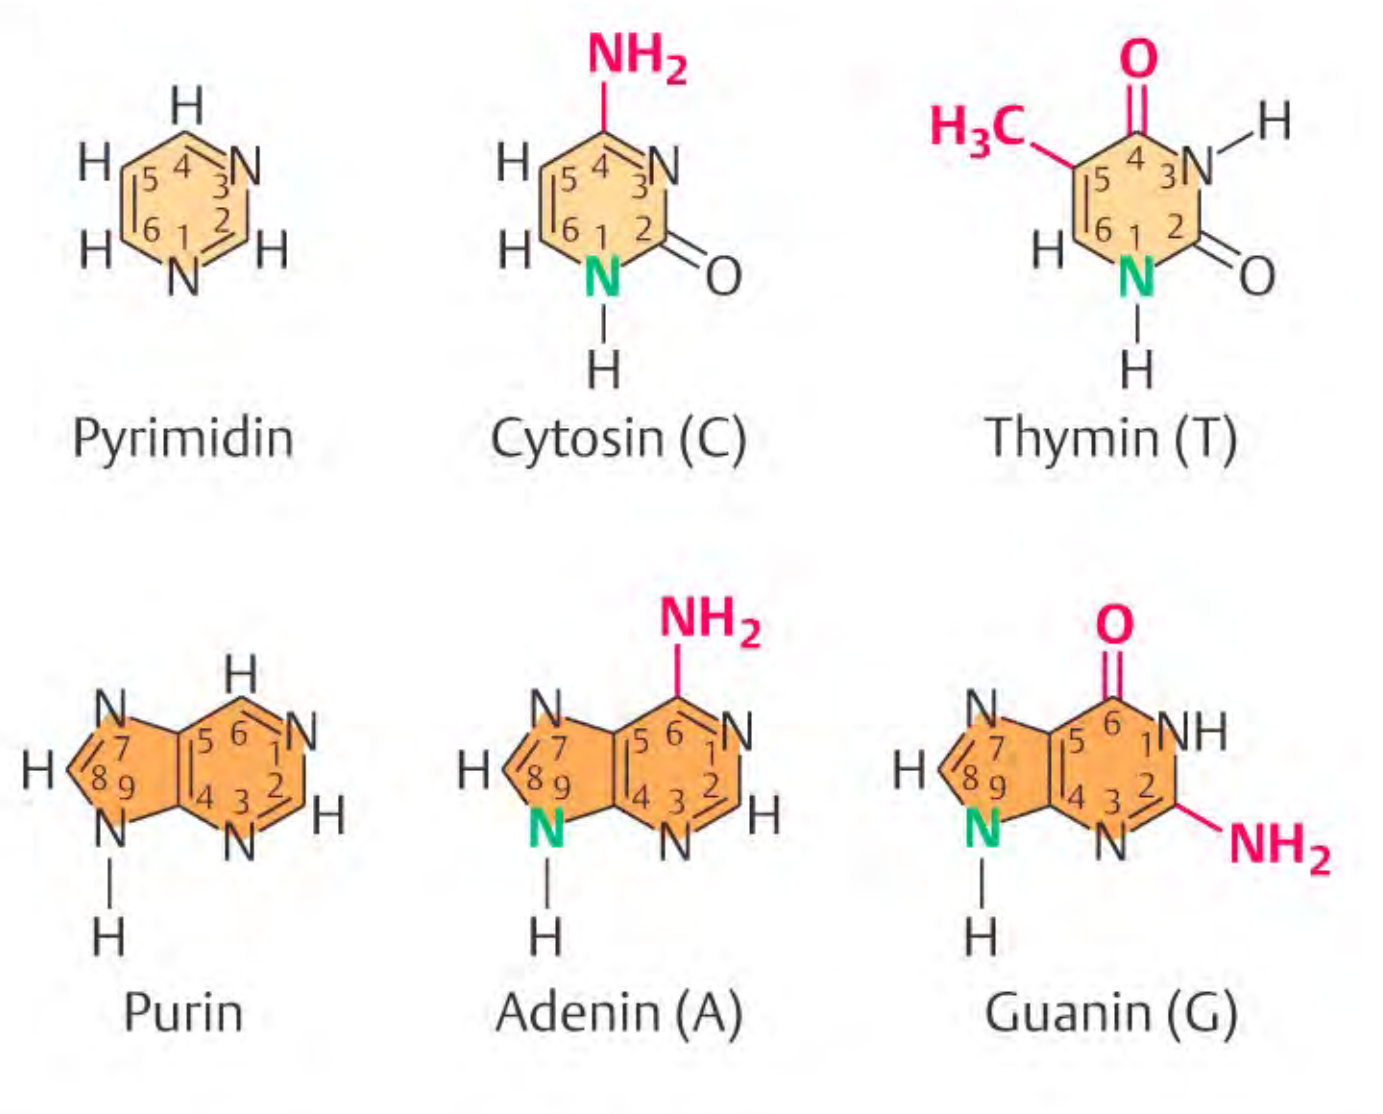
\includegraphics[width=\textwidth]{bilder/basen}
    \caption{Die Schmelzkurve der DNA}\label{fig:figure}
\end{figure}

\defin{cot_analyse}

\section{Das Genom}\label{sec:das-genom}

\defin{genom}

\defin{nukleom}

\defin{plastom}

\defin{chondrom}

\section{DNA-Replikation}\label{sec:dna-replikation}

\defin{konRep}
\defin{disRep}
\defin{semiRep}

\defin{biRep}

\subsection{Start der Replikation}\label{subsec:start-der-replikation}
\defin{oric}

\begin{figure}[H]
    % TODO F26 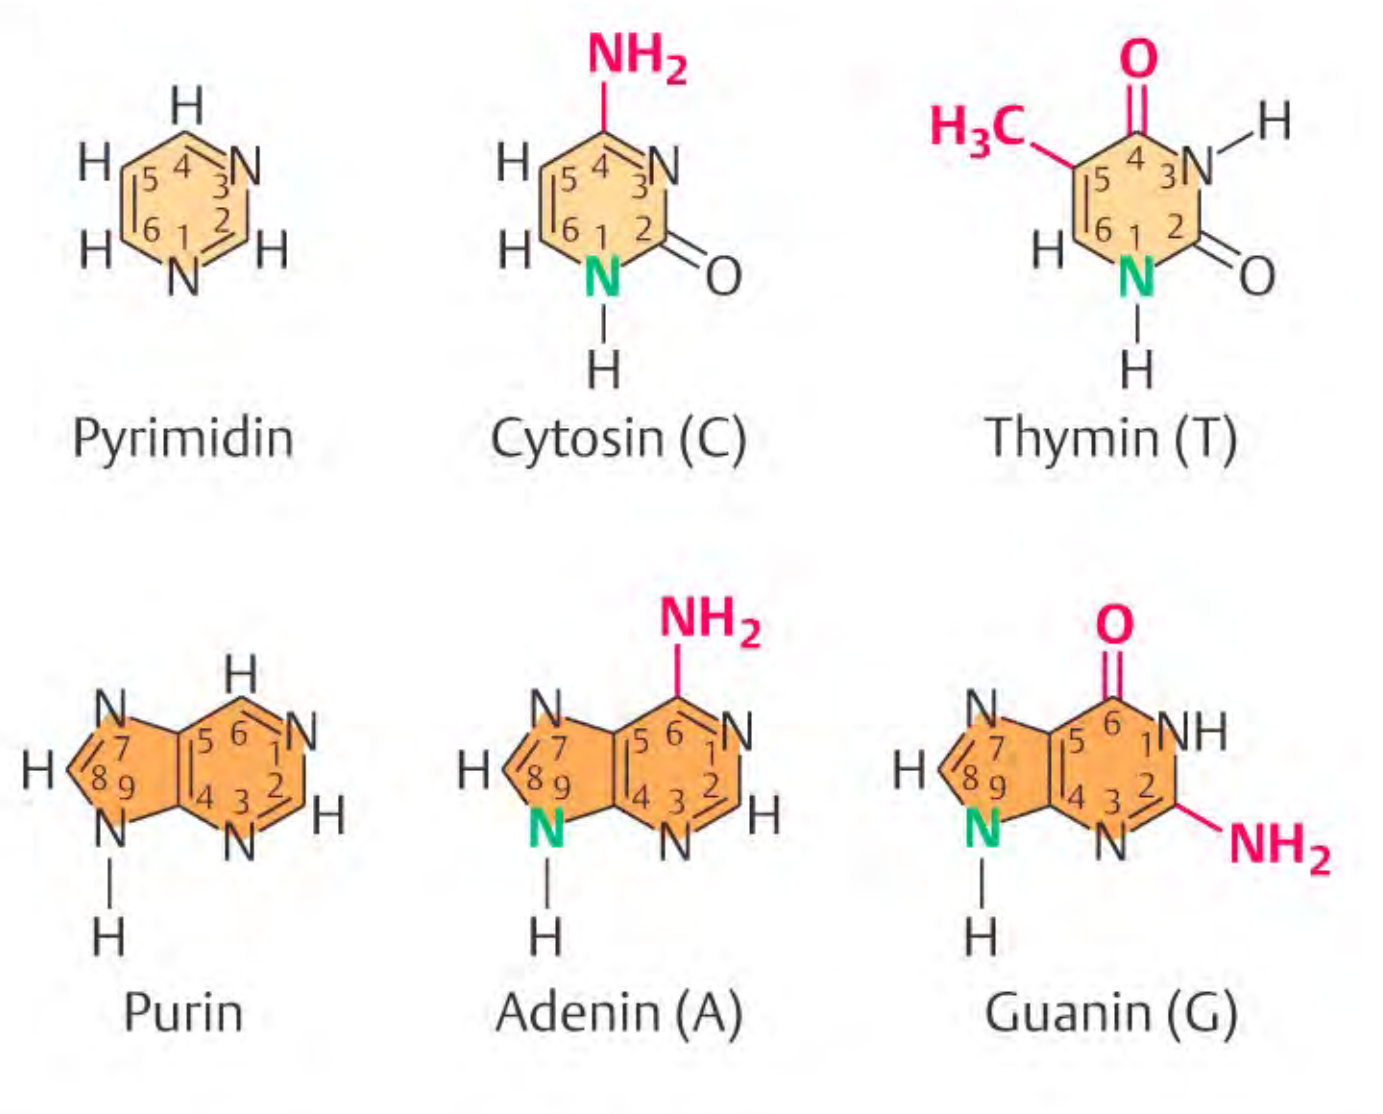
\includegraphics[width=\textwidth]{bilder/basen}
    \caption{Start der Replikation am oriC.}\label{fig:figure2}
\end{figure}

\subsection{DNA-abhängige DNA-Polymerase}\label{subsec:dna-abhangige-dna-polymerase}

Alle DNA-Polymerasen benötigen einen Primer\ldots
% TODO F27

\subsection{Die Replikationsgabel}\label{subsec:die-replikationsgabel}
% TODO F28, 34

\subsection{Primase und DNA-Polymerase III}\label{subsec:primase-und-dna-polymerase-iii}
% TODO F32-33, 35

\subsection{Die DNA-Polymerase I}\label{subsec:die-dna-polymerase-i}

\begin{bsp}
    \textbf{Die DNA-Polymerase I von E. coli}
    % TODO 38 - 43
\end{bsp}

\subsection{Weiterer Verlauf der Replikation}\label{subsec:weiterer-verlauf-der-replikation}

% TODO 60-63

\subsection{Abschluss der Replikation}\label{subsec:abschluss-der-replikation}


\section{DNA-Superhelikalität}\label{sec:dna-superhelikalitat}

% TODO F 49 - 55, 60

\begin{bsp}
    \textbf{Replikation des Escherichia coli-Chromosoms}
\end{bsp}

\section{DNA Topoisomerasen}\label{sec:dna-topoisomerasen}

% TODO F 56-58
